\documentclass[a4paper, 11pt]{article}
\usepackage{epsf}
\usepackage{epsfig}
\usepackage{amsmath}
\usepackage{amssymb}
\usepackage{theorem}
\usepackage{alltt}
\usepackage{times}
\usepackage{helvet}
\topmargin=15pt
\oddsidemargin=20pt
\headsep=20pt
\footskip=30pt
\textheight=600pt
\textwidth=400pt

\renewcommand{\familydefault}{\sfdefault}

\begin{document}
\title{The {\tt NestedMICA} motif inference tool}
\author{Thomas A. Down \\ 
  {\it thomas.a.down@googlemail.com}}
\date{Version 0.8.0 [20070425]}
\maketitle

\begin{abstract}
NestedMICA is a sensitive, scalable, pattern-discovery system, aimed at finding
transcription factor binding sites and similar motifs in biological sequence.
More discussion of the principles behind NestedMICA, and an evaluation of
its sensitivity can be found in a recent paper \cite{down.nmica}.

If you have any problems or questions about the system, please contact Thomas Down.
\end{abstract}

\section{Theory}

Motif-finding is a long standing problem in sequence bioinformatics.
A typical statement of the problem would be ``given a set of
sequences, which motifs are significantly over-represented with
respect to a given model of non-functional sequence.''  The choice of
non-functional sequence (background) model is an important part of
this question and will be discussed in more detail later.  The
classical use for motif-finding software is the detection of
transcription factor binding sites in promoter regions, but there are
other interesting functional elements in biological sequences and
elsewhere which can be found by motif-discovery methods.

Motif-finding strategies can be broadly divided into two classes: methods which
rely on exhaustively enumerating a set of motifs (generally using an optimized
data structure such as a suffix tree) then reporting the most frequently occuring, and methods
which find significant motifs by optimizing or drawing samples from a probabilistic
model.  Exhaustive enumeration is a good strategy for finding perfectly conserved
motifs ({\it i.e.} every instance is identical), but for typical transcription
factor binding sites, which often have several weakly constrained positions,
exhaustive enumeration becomes problematic and the results usually have to be
post-processed with some kind of clustering system.  NestedMICA is a probabilitic
motif finder, and we will not consider exhaustive enumeration further.

Probabilistic motif-finders treat the supplied sequences as a mixture of `interesting'
motifs and `non-interesting' background sequences.  This problem has classically
been reduced to a simple case: considering just one motif at a time, model each
sequence with a random background model which may, or may not, contain a single
instance of the motif under consideration.  This is the zero-or-one occurance per sequence
(ZOOPS) model.  It can be easily represented as a hidden Markov model (figure \ref{zoops.smm})),
and standard techniques such as expectation maximization \cite{bailey.meme} or 
Gibbs sampling \cite{thompson.gibbs} can
be used to find good sets of model parameters (corresponding to good motif models).

\begin{figure}[!bth]
\begin{center}
\includegraphics[scale=0.66]{memehmm.pdf}
\caption{The ZOOPS sequence mixture model}
\label{zoops.smm}
\end{center}
\end{figure}

There are two significant concerns about this strategy which NestedMICA tries
to address:

\begin{itemize}

\item{Real regulatory regions, and most other contexts where interesting motifs
can be found, don't really contain just a single instance of a single motif.
Programs which use the ZOOPS model work around this by finding the strongest
motif in a set, then scanning for all its instances, masking them out, and re-running
the process on the remaining sequence.  This strategy is greedy and it is by no
means clear that its behaviour will be optimal, especially when working on a
system where there is a set of closely related, yet still distinct, motif types.
In an environment where novel transcription factors are created by gene duplication
then diverge to perform a new function, such situations seem quite probable, and
have not yet been well investigated.}

\item{Existing techniques for optimizing or exploring sequence models of this
type tend to be strongly local in nature -- they concentrate on regions of the
probability landscape close to their starting point.  This is particularly clear for
expectation-maximization methods, which always move in a direction which increases the
likelihood of the model.  Sampling strategies don't strictly have this limitation, 
but in practice, crossing the low-likelihood valley between two high-likelihood
peaks is unlikely, often to the point where it becomes vanishingly rare.}

\end{itemize}

\subsection{Motif ICA}

We treat finding multiple motifs in a set of sequences as a form of independent component
analysis (ICA) problem.  In linear ICA, a matrix of observations, $X$ is approximated
as a linear mixture, $A$ of some sources, $s$:

\begin{equation}
x = As + \nu
\end{equation}

(where $\nu$ is a noise matrix).  A classical example is the ``cocktail party problem'' where
a set of $M$ microphones record different mixtures of the voices of $N$ speakers.  Given
samples from these microphones at $t$ timepoints, ICA attempts to factorize the $M \times t$
observation matrix into a $N \times t$ source matrix and a $M \times N$ mixing matrix.

It is possible to generalize ICA to {\em any} mixing situtation, given a suitable
mixing operator.  In the classical case, the mixing operator is simply the addition
operator.

In motif ICA, the sources are short sequence motifs (currently, but not necessarily,
modeled as position-weight matrices \cite{bucher.wms}), while the observations are larger sequences.
There are a number of interpretations of the mixing matrix.  Currently, we use a
boolean mixing matrix (all coefficients are either 0 or 1), and a given sequence
is expected to contain a given motif if the relevent mixing coefficient is 1.  The
`noise' part of the ICA model represents all the sequence which isn't modelled by
one of the motifs.

\subsection{Nested sampling}

Nested sampling is an alternative way of performing probabilistic inference in a
Bayesian framework, proposed recently by John Skilling \cite {skilling.nested}.  It can be
considered to be a Monte Carlo method, since the process is driven forward by
a series of randomly chosen events, but it is quite distinct from the classic
Metropolis-Hastings method, and methods such as Gibbs sampling and slice samplings,
which can all be considered as optimized implementation strategies for Metropolis-Hastings.

Nested sampling is applied to an {\it ensemble} of states, which represent possible
solutions to the problem at hand.  The ensemble is initialized by sampling uniformly
from the prior distribution, then sorting the states according to their likelihoods.
In nested sampling, Each state in the ensemble is considered to be a representative of the set of states 
with similar likelihoods.  If the likelihood of each state is drawn as a contour on
the likelihood distribution, we see a nested set of contour lines, converging towards
the peaks of the likelihood distribution.  We therefore call the ordered set of states
a nested ensemble.  For each cycle of nested sampling, the least likely state in the
ensemble is discarded, and a new state is chosen by sampling uniformly from the prior
subect to the constraint that the likelihood of the new state must be greater than or
equal to the likelihood of the discarded state.

In this context, the most exciting property of nested sampling is that, given a
reasonably large ensemble, the final sample drawn from a converged nested sampler
can be expected to reflect the global optimum of the likelihood landscape.
Moreover, in cases where more than one globally significant optimum exists, these
should be represented in the sample set in direct proportion to the amount of
posterior mass they represent.

\subsection{Background models}

The background model is an important component of the SMM framework -- after all,
it will usually be responsible for modeling the majority of the input sequence!
The simplest strategy -- and still a common one -- is to treat all non-motif sites
as independent and identically distributed.  In HMM terms, this makes the background
model a zeroth-order Markov chain.  However experience shows that genomic DNA 
sequence, even when apparently totally non-functional, is not a good fit to the
i.i.d. model.  The best known deviation is perhaps the dramatic under-representation
of CpG dinucleotides in most parts of vertebrate genomes, but other significant
effects are known.  In any case, practical experience shows that motif finders
equipped with naive background models tend to report low-complexity elements rather
than interesting binding sites.

The first obvious improvement is to replace the zeroth order Markov chain with
a first order chain ({\it i.e.} the probability of observing a particular symbol
at position $n$ depends on the symbol at position $n-1$).  This model is good at
capturing anomalies like the CpG underrepresentation.  The success of first
order background models has led some researchers to investigate higher order models.
One investigation of Markov chain backgrounds can be found in \cite{thijs.background}: this concludes
that pentanucleotide frequency tables ({\it i.e.} fourth-order background models)
are optimal.  However, there are two concerns about this result: firstly, it
leaves an open question about what these high-order correlations in background
sequence mean (and why fourth-order models appear to outperform fifth-order).  Also,
training a background model generally requires sequence propoortional to the number
of free parameters in the model.  Fifth order models, with 768 parameters, therefore
require large amounts of sequence.  Moreover, it is desirable to train the background
model on sequence which does not contain target motifs, since a fifth order model
could easily capture some information about this motifs, thereby reducing the
sensitivity of the motif-finding process.  But it is hard to find large amounts
of representative background training sequence which doesn't contain interesting
motifs.

A different way to generalize the naive background model is to allow several
different classes of sequence, each with its own particular base distribution
(which could be zeroth-order or higher-order).  We call these {\it mosaic models},
since their underlying assumption is that genome evolution includes some set of
constraints which act non-uniformly, even on background sequence.

To investigate the benefit of mosaic models, we took a set of human upstream
flanking regions, and split the set in half, using one subset to optimize the
background model parameters and the second subset for testing.  Test likelihoods
for a variety of class numbers and Markov chain orders are shown in figure
\ref{mosaic.fit}.  Considering one class `mosaics' (which are equivalent to
uniform background models), we repeat the previously reported observation that
higher order Markov chains are better models of genomic DNA.  However, we also
see large increases in likelihood when moving to larger numbers of mosaic classes.
Interestingly, the lines for zeroth-order and first-order models run almost
paralell: this suggests that the benefits of mosaic models are almost orthogonal
to the benefits of first-order models.  However, this is not true when moving
beyond first-order models.

\begin{figure}[!bth]
\begin{center}
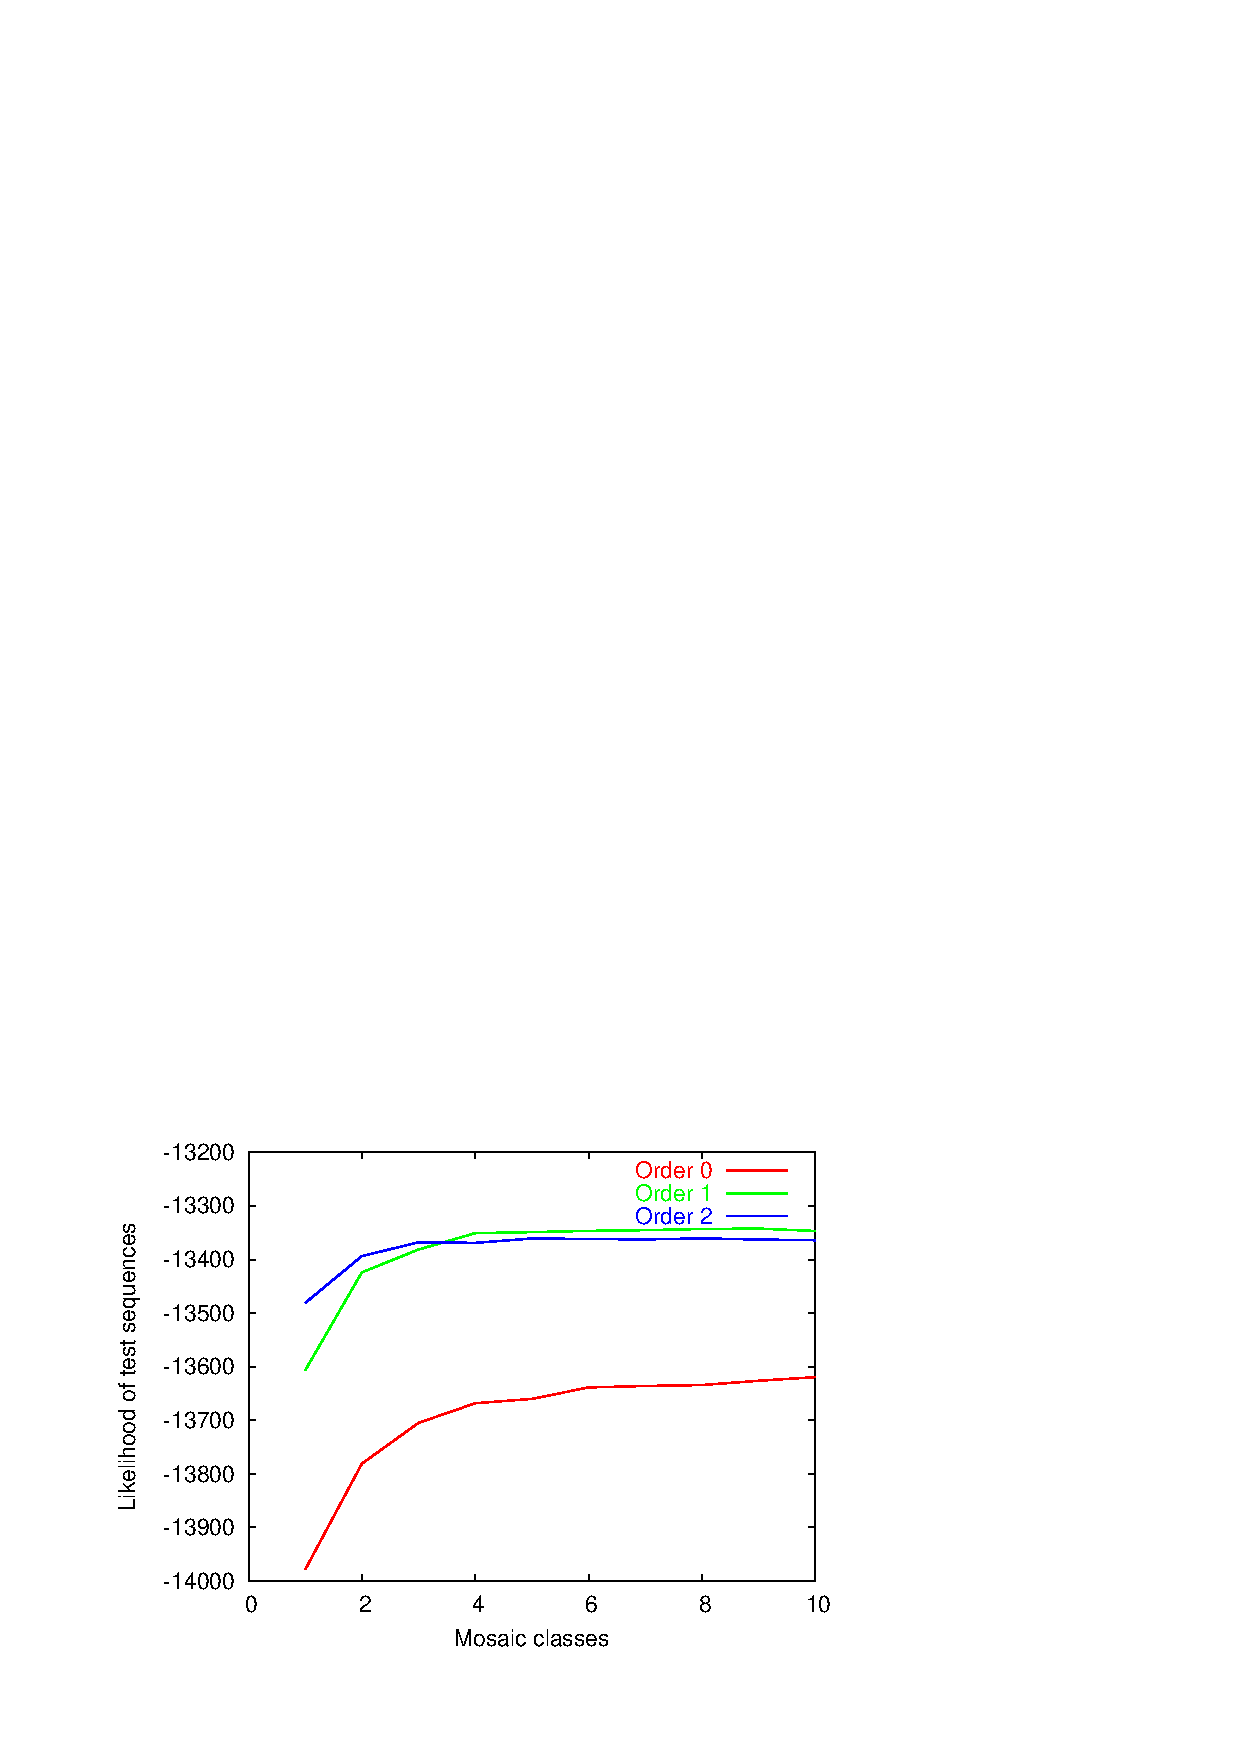
\includegraphics[scale=0.8]{mosaic-fit.pdf}
\caption{Comparison of mosaic backgrounds}
\label{mosaic.fit}
\end{center}
\end{figure}

Based on these results, we recommend the use of a four class, first order, mosaic
background model for most motif-finding applications on mammalian genomic sequence.
In practice, the four classes appear to be:

\begin{itemize}

\item {A relatively neutral class}

\item {A C+G rich class (CpG islands?)}

\item {Purine rich}

\item {Pyrimidine rich}

\end{itemize}


There are still open questions about the biological significance of the mosaic classes
we have observed.

\section{Running NestedMICA}

NestedMICA is open source software, released under the GNU Lesser GPL.  The
main program is written in Java, but there are a few small pieces of native C
code which are required.  The C code is simple and (hopefully) portable, so it
should be possible to run NestedMICA on most modern computer platforms.

The NestedMICA source distribution can be downloaded from

\begin{alltt}    http://www.sanger.ac.uk/Software/analysis/nmica/\end{alltt}
This distribution includes all the required library code.
To compile the Java code, you'll
need version 1.7.0 or later of the ANT java build tool, which can be downloaded from
{\tt http://ant.apache.org/}.

As of NestedMICA 0.7, a Java 5 runtime environment is required.  In
general, we recommend that you use the latest available Java from Sun
Microsystems.  Initial benchmarks suggest that Java 6 runtimes run
NestedMICA about 10\% faster, so use the latest version if it's
available.  Mac OS X is a supported platform, but you'll need to run
version 10.4.0 (``Tiger'') or later, and separately download the Java
5 packages from Apple.  You'll also need to reconfigure your system to
make Java 5 the default version for command-line applications (note
that Apple's Java Preferences tool doesn't do this, it only affects
programs started via your web browser).  The best way to do this is to
add the following lines to the {\tt .bashrc} file in your home
directory:

\begin{alltt}    export JAVA\_HOME=/System/Library/Frameworks/JavaVM.framework/
                      Versions/1.5.0/Home
    export PATH=\$\{JAVA\_HOME\}/bin:\$PATH\end{alltt}

\subsection{Building and installing NestedMICA}

NestedMICA is written in the Java programming language, with a small amount of C
used for performance reasons.  On supported platforms, it should be possible to
compile the whole system by typing {\tt ant} at the command line.  If this
does not complete cleanly, contact Thomas Down with the complete error message
and details of the platform you're running on.
      
Currently supported platforms are Linux and Mac OS X, but other
Unix-like platforms may also work, and if not it should be reasonably
easy to add support.  Note that we've had reports of problems when
building on Mac OS with old developer tools (before gcc version 3.1).
If in doubt, please install the latest developer tools.

Once you have compiled NestedMICA successfully, you can either add it
directly to your PATH:

\begin{alltt}    export PATH=/home/thomas/nmica-X.Y.Z/bin:\$PATH\end{alltt}

or copy it to some other location.  If you are packaging NestedMICA or building
it for other users, only the {\tt bin}, {\tt lib}, and {\tt native} subdirectories
are required once NestedMICA has been compiled.

\subsection {Basic operation}

This section describes a (very) small set of test sequences named {\tt micatest100.fa} 
which are included with the NestedMICA source
distribution.  The file contains 100 synthetic DNA sequences, each of
50 bases long.  The set contains two spiked-in motifs.

The main part of NestedMICA is the motif inference tool, {\tt nminfer}.  You
should be able to recover the two spiked motifs using a command like:

\begin{alltt}    nminfer -seqs micatest100.fa -numMotifs 2 
            -minLength 4 -maxLength 12 -ensembleSize 50\end{alltt}
    
This runs the motif finding system until the nested sampling process is
close to convergence, then writes the optimal set of motifs to a file
named {\tt motifs.xms}.  In this case, we're telling {\tt nminfer} that
we expect to find 2 motifs, but setting a fairly broad range of possible
motif lengths.

You can view your discovered motifs using the MotifExplorer tool, available
from:

\begin{alltt}    http://www.sanger.ac.uk/Software/analysis/nmica/mxt.shtml\end{alltt}

\begin{figure}[!bth]
\begin{center}

\includegraphics[scale=0.66]{mt100-motifs.png}
\caption{Motifs discovered from the demonstration set.}
\label{example.motifs}
\end{center}
\end{figure}

One word of warning here: the {\tt -ensembleSize 50} option is recommended here
in order to get quick results on this simple test data set, but will lead to lower
sensitivity than leaving {\tt -ensembleSize} at its default value.  For normal
use, we do not recommend altering {\tt -ensembleSize} from its default value.

\subsection {Increasing the memory limits}

Some Java implementations may, by default, limit NestedMICA's memory usage to an unreasonably
small value.  If NestedMICA is crashing with {\tt OutOfMemoryError}, you can explicity set a
new memory limit by setting an environment variable.  To set the memory limit to 500Mb, use:

\begin{alltt}    export NMICA_JVMOPTS=-Xmx500M\end{alltt}

As a rough rule-of-thumb, a good memory limit for large datasets is 1Mb of memory for every
1Kb of input sequence.  Note that just because you have allocated NestedMICA 500Mb of
memory using a command like that shown above, it won't immediate use all that memory --
it just specifies how much memory the program is allowed to use before exiting.

\subsection{Background-model options}
\label{background}

By default, {\tt nminfer} will build a background model from the supplied sequences.
The default model is quite simple: a single zeroth order ({\it i.e.} mononucleotide
frequencies) model for all the input sequences.  You can specify more complex models
using the {\tt -backgroundOrder} and {\tt -backgroundClasses} options.  So to use a
four-class dinucleotide model (which seems to be a good choice for vertebrate
sequences) you could use:

\begin{alltt}    nminfer ... -backgroundOrder 1 -backgroundClasses 4 ...\end{alltt}

However, complex background models can take some time to train, and it is useful
to be able to run nminfer multiple times using exactly the same background.
Therefore, we recommend building background models as a separate step, {\it e.g.}:

\begin{alltt}    nmmakebg -seqs seqfile.fa -order 1 -classes 4
             -out background42.xml\end{alltt}

The resulting background model is stored as an XML file which can be inspected if
you want to see the exact parameters that have been chosen.  Having built a
background model in this way, you can use it for any motif finding run:

\begin{alltt}    nminfer ... -backgroundModel background42.xml ...\end{alltt}

Remember that if you run {\tt nminfer} in this way, the {\tt -backgroundOrder}
and {\tt -backgroundClasses} options will be silently ignored -- the background model
architecture is hardwired when the model is trained.

{\bf Note:} earlier versions of NestedMICA used a different file format for
storing background models.  You can convert these old files into the new XML
format using {\tt nmconvertbg}:

\begin{alltt}    nmconvertbg -in background42.sbg -out background42.xml\end{alltt}

\subsection{Background model architecture optimization}
\label{bg-optimize}

Our experience suggests that a background model trained with the parameters
{\tt -order 1} and {\tt -classes 4} is generally a good choice when working
with vertebrate genomes.  However, genome composition varies between species
and it is likely that other architectures may be better choices in some cases:
for example, a six-class model was used in a recent study of the insect
{\it Drosophila melanogaster} \cite{down.tiffin}.  One principled approach to background selection
might be to repeat the experiment depicted in figure \ref{mosaic.fit} using
sequences from your species of interest.  To do this, take a set of sequences
(ideally around 200), then:

\begin{alltt}    nmevaluatebg -seqs seqs.fa -order 1 >eval.dat\end{alltt}

The {\tt nmevaluatebg} splits the sequences into two sets -- by default
it places 50 sequences in the ``test'' set and the rest in the
``training'' set.  It fits background models with varying numbers of
classes to the training sequences, then calculates the likelihood of
observing the test sequences under the newly-trained model.  If you plot
the output using a tool like {\tt gnuplot}, you should see a plot similar
to one of the lines shown in figure \ref{mosaic.fit}.  Look for a 
plateau in this plot: the class number on the shoulder of the plateau
should represent a good trade-off between background model complexity
and fitting the date well.

It is also possible to use {\tt nmevaluatebg} to compare different values
of the {\tt -order} parameter, by running the program serveral times then
comparing the output.  This has a few complications: firstly, you must
ensure that the ``test'' and ``training'' sets are the same for all runs.
To do this, split the sequences up manually then use the {\tt -trainSeqs}
and {\tt -testSeqs} options.  Also, it is necessary to compensate for edge
effects: when working with an order 2 background model, NestedMICA can't
``see'' the first two bases of each sequence, therefore the likelihood
of the sequence set will appear to be higher.  You can compensate for
this using the {\tt -trim} option when testing low-order background models,
{\it e.g.}:

\begin{alltt}    nmevaluatebg ... -order 0 -trim 2 >order0.dat
    nmevaluatebg ... -order 1 -trim 1 >order1.dat
    nmevaluatebg ... -order 2 >order2.dat\end{alltt}

\subsection {Motif-finding options}

The {\tt nfinfer} program has many options.  You can see a list of common options
by typing {\tt nminfer -help}.

\subsection {Everyday options}

These are options that you'll use all the time, and are generally well-behaved.

{\tt -numMotifs {\it n}} specifies the number of motifs you want to find (default=1).

{\tt -maxLength {\it n}} the maximum length of motifs to find (default=10).

{\tt -minLength \it{n}} the minimum length of motifs to find (if not specified, a 
warning will be printed and this will be set equal to {\tt -maxLength}).

{\tt -seqs \it{filename}} a FASTA-formated database of sequences to analyse.

{\tt -backgroundModel \it{filename}} the background model to use, normally generated
by running the {\tt nmmakebg} program.

{\tt -out \it{filename}} name of a file to write the final motif set (default
{\tt motifs.xms})

{\tt -sampleFile {\it filename}} name of a file to write periodic samples during
the motif-finding process.  If you run the finder with the option {\tt -sampleFile foo},
it will write sample files {\tt foo.1000.xms}, {\tt foo.2000.xms}, etc.

{\tt -sampleInterval {\it n}} number of cycles between sample files (default=1000).

{\tt -maxCycles {\it n}} the maximum number of cycles to run the sampler.  The program
will then exit regardless of convergence status.  Currently the criteria for deciding
when the process has converged are quite conservative, so this option may be useful.

{\tt -ensembleSize \it{n}} the size of the nested ensemble used to explore the probability
landscape.  Larger values improve reproducibility at the expense of speed.  Default behaviour
is to set the ensembleSize to 200 for large problems ($>=5$ motifs), but to use larger ensemble
sizes when learning less motifs, up to a maximum of 1000 when learning a single motif.  This
should give maximum sensitivity under most circumstances.  When learning one or two motifs
from a very simple dataset, you may want to explicitly force a small ensembleSize for
performance reasons.

{\tt -alphabet (dna|protein)} the alphabet of input sequences.  Default is DNA.

{\tt -revComp} allow motifs to occur in either orientation (off by default, slows the program
down by a factor of about 2).

{\tt -cluster} prefer motifs which occur in clusters.  Causes a small slowdown in training.
Currently not sure how helpful this is.

\subsection {Advanced options}

More complex options, that we'd prefer weren't there.  If you're interested in these, it's
probably best to discuss them with Thomas Down.

{\tt -mixtureType (binary|flat|logit|weighted)}  Wierd switch which effects the interpretation of
the mixing matrix.  Default is {\tt binary}, leave it that way unless you know what you're
doing.

{\tt -mixtureUpdate (resample|weakResample|max|queue|random)}  Strategy for updating the mixing
matrix during training.  {\tt resample} is the best in theory and works well for most problems.
{\tt weakResample} gives better results on large sets of human promoters.  Don't use any of
the others.

{\tt -expectedUsageFraction {\it d}} number between 0.0 and 1.0 giving the prior belief of
motif frequency.  Default is 0.5.  Try 0.1 if you think motifs are rare, 0.9 is you think almost
all the sequences are likely to contain an instance.

{\tt (-counted|-uncounted)} switch between a model where a motif can occur any number
of times in a sequence (uncounted), and a more conventional motif-inference strategy
where motif-containing sequences are expected to contain exactly one occurence.  Note
that the {\tt -counted} model is slower, and is likely to become unusably slow with
values of {\tt -numMotifs} greater than about 5.  However, it may be preferred in some
situations where sensitivity is paramount.  Default is {\tt -uncounted}.

\subsection {Checkpointing}

To minimize the risk of data loss during long runs, NestedMICA can generate
checkpoint files at regular intervals during the training process.  If you want
to keep checkpoint files, add the following arguments to your {\tt nminfer}
command line

\begin{alltt}    -checkpoint mycp -checkpointInterval 1000\end{alltt}

Like sample files, checkpoints are automatically numbered with the cycle number
at which they are taken.  Unlike samples they files are rather large (typically
several megabytes, increasing rapidly with dataset and nested ensemble size).  By
default, {\tt nminfer} deletes old checkpoints: in the standard configuration
only two checkpoints are kept on disk, so after the third is written, the first
will be deleted.  This behaviour can be changed using the {\tt -keepCheckpoints}
option.

To restart from a checkpoint:

\begin{alltt}    nminfer -restartFromCheckpoint mycp.12000.jos 
            -maxCycles 100000 -sampleFile sample -sampleInterval 10000 
            -checkpoint mycp2 -checkpointInterval 1000\end{alltt}
    
Note that, while the entire trainer state is restored from the checkpoint file,
currently none of the `housekeeping' options (termination, sampling, and checkpointing)
are, so it is necessary to re-specify them when restarting the checkpoint.  This
is potentially useful if you want to continue the training of a run which hasn't
quite converged for a few extra cycles.

\subsection {Multithreaded operation (SMP machines)}

If you are running on a multi-processor machine, add the option {\tt -threads N}
to the {\tt nminfer} command line, where {\tt N} is the number of processors
in the machine, or the number of CPUs in a large multiprocessor server that you
want to devote to {\tt nminfer}.  This mode of operation is quite efficient,
usually giving better than 95\% scaling from one to four processors.  This option
should also work efficiently on large SMP machines, at least when working with large
datasets, but has not been tested extensively with more than 4 CPUs.

\subsection {Distributed operation (clusters, farms, Beowulfs, etc.)}

An alternative approach to paralelizing a large {\tt nminfer} run is distribute
the workload over multiple nodes.  Start {\tt nminfer} as usual, but add the
options:

\begin{alltt}    -distributed -port XXXXX\end{alltt}
      
You may use any port number between 1024 and 65535, but if you are running
multiple {\tt nminfer} jobs on one cluster, you should give each job a
unique port number.  This process will be your {\it master node}.  Once it has
started up, you can run any number of {\it worker nodes}, which will evaluate
sub-problems for the master node.  To run a worker node:

\begin{alltt}    nmworker -server YYYYY -port XXXXX\end{alltt}
     
Where {\tt YYYYY} is the name (or IP address) of the master node, and the port
number matches that used to start the master.  To remove a worker node from the
cluster you can simply kill the process.  It's fine to add and remove
workers at any point during the run, although there is currently a short
(\~10 seconds) glitch after a worker dies during which no work will be done, so very
rapid worker turnover can be inefficient.  If
the {\tt nminfer} run ends normally, all associated worker nodes will be sent
a shutdown message, but under other circumstances it may be necessary to kill
worker nodes manually.

In NestedMICA 0.7.x, the master node did not perform much computation,
and was restricted to housekeeping tasks.  As of NestedMICA 0.8.0, you can
{\it optionally} use the master node as an extra compute node.  To do this, you
should explicitly specify a {\tt -threads} option when starting the {\tt
nminfer} process.  Depending on the hardware you are using and the number
of worker nodes you have attached, the optimum value will be either $n$ or
$n-1$ where $n$ is the number of CPUs in your computer.  Using a value of
$n$ will maximize CPU utilization, while a value of $n-1$ leaves one CPU core
free at all times for housekeeping tasks.  If you run a lot of distributed
{\tt nminfer} processes, it is worth doing some testing to find the optimum
value for your cluster.

\subsection{Comparative genomics}

If groups of orthologous regulatory regions are available, NestedMICA can take advantage
of the known relationships between species.  Unlike phylogenetic footprinting and other
`infinite monkeys' techniques, comparative NestedMICA does not consider the alignments
of the sequences, but simply assumes that orthologous regulators are likely to contain
similar complements of motifs.  In practice, this is implemented by using a single
row of the ICA mixing matrix to model all the orthologs.

To run NestedMICA in comparative mode, just add more than one {\tt -seqs} option to
the {\tt nminfer} command line.  If two sequences in different files share the same
name, they will be treated as orthologues.

There are two options for providing background models in comparative mode.  If only
one {\tt -backgroundModel} switch is present on the command line, that single background
model will be used for all species.  Alternatively, you can train a separate background
model for each species, and specify them with multiple {\tt -backgroundModel} switches,
e.g.

\begin{alltt}    -seqs human.fa -backgroundModel human.sbg 
    -seqs mouse.fa -backgroundModel mouse.sbg\end{alltt}

If you use multiple background models they {\it must} be listed in the same order as
the sequence databases, and there must be exactly equal numbers of sequence databases
and background models.  If no background models are supplied, a separate background model
will be constructed for each supplied sequence file.

If ortholog information is only available for some sequences, that's fine.

There is no limit to the number of species that can be used (except for practical
memory limits).  We would expect to see diminishing returns beyond about 4 species,
but much more testing is needed to determine the optimal configurations.

\subsection{Scanning with motifs}

A simple program is supplied to scan a sequence using weight matrices inferred by
NestedMICA.  Hits are output in GFF format.  This program uses bits-sub-optimal
scoring: this means that the best possible match to a given weight matrix will
always score 0.0, while other sequences will receive negative scores.

Typical usage:

\begin{alltt}    nmscan -seqs seqfile.fa -motifs motifs.xms
           -scoreThreshold -5.0 -strand both\end{alltt}

\section{Using NestedMICA for protein motif discovery}
\begin{alltt}\emph{--by Mutlu Do\={g}ruel, md5@sanger.ac.uk}\end{alltt}

As of version 0.7.3, NestedMICA is capable of finding motifs in protein sequences \cite{dogruel.nmica}.  For protein analysis, each NestedMICA tool ({\tt nminfer}, {\tt nmevaluatebg}, {\tt nmmakebg}, etc.) must be run with the {\tt -alphabet protein} option. While the underlying principle remains the same as DNA motif finding, some extra care must be taken during background model training and parameter choice.

\subsection{Background optimization and training}

Experience suggests that protein sequences are complicated enough to
prevent us from easily saying that a pre-determined number of mosaic
classes or background order would be optimal. Most of the time,
training a dedicated background model for each protein sequence set is
needed to maximise performance and sensitivity.

As described in Section \ref{bg-optimize}, in order to find a reasonable pair of order and class number for background creation, it is possible to use a build-in application called nmevaluatebg. If you divide your data into two parts, you can use {\tt nmevaluatebg} in the following way:

\begin{alltt}    nmevaluatebg -trainSeqs proteinsTrain.fa 
                 -testSeqs proteinsTest.fa 
                 -alphabet protein -order 0
                 -minClasses 1 -maxClasses 7\end{alltt}

Unless {\tt -trainSeqs} and {\tt -testSeqs} parameters are used, NestedMICA will randomly use a certain number of sequences from a dataset provided with the {\tt -seqs} option. This would not be ideal if, for example, you would like to compare the likelihood of an order-1 background with a previous run.

\begin{figure}[!bth]
\begin{center}
\includegraphics[scale=0.5]{proteinEval.pdf}
\caption{Likelihood curve for protein background models with different number of mosaic classes.}
\label{proteinEval}
\end{center}
\end{figure}

While, in principle, using higher orders and larger number of mosaic classes would fit the data better and better, this will not hold true after a while when there is no sufficient data to train a more complicated model properly. Generally, it's a good idea to pick a class number before the likelihood curve starts to drop, no matter of it is increasing at a later stage. Figure \ref{proteinEval}, for example, shows the values of an nmevaluatebg optimization for a small protein set. In this particular case, choosing 5 or 4 mosaic classes would be a safer option and more optimal.

Having found a good pair of parameters, a background model is trained in a similar way as described in Section \ref{background}:

\begin{alltt}    nmakebg -seqs proteins.fa -order 0 -classes 4 
            -alphabet protein -out proteinbg.xml\end{alltt}

\subsection{Motif finding options}

While all user parameters remain the same, a small number of NestedMICA parameters have different default values for proteins. {\tt -ensembleSize} is the most notable one:

When searching for up to 3 motifs, the default behaviour is to set the {\tt ensembleSize} to 1500 divided by the number of motifs. When more number of motifs are searched, it is set automatically to 500, unless there is a user specified value. This parameter can affect the speed of the program dramatically.

\bibliographystyle{nmica}  % Style BST file
  \bibliography{nmica}

\end{document}
